\documentclass[a4paper,10pt]{article}
\usepackage[utf8]{inputenc}
\usepackage[francais]{babel}
\usepackage[top=4cm, bottom=4cm, left=2cm, right=2cm]{geometry}
\usepackage{alltt}
\usepackage{graphicx}

\title{\textbf{Projet d'Algorithmique Réparti Avancé}}
\author{}
\date{29 octobre 2013}

\begin{document}
\maketitle
\newpage

\paragraph{}\fbox{\begin{minipage}{1\textwidth}\textbf{Question 1} \textit{Draw a picture showing a Z-configuration on a square O-Grid of side 7. By convenience, design your picture using a grid representation (see for instance Figures 2 and 3).}
\end{minipage}}
\paragraph{}

\begin{figure}
   \centering
   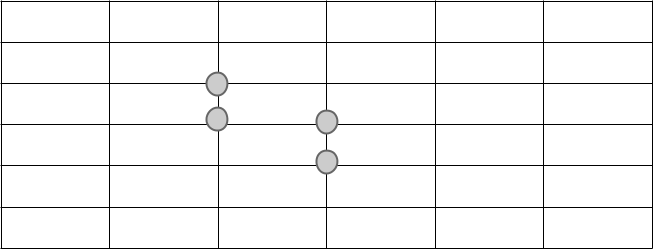
\includegraphics[scale=0.6]{images/question_1.png}
   \caption{Une Z-Configuration sur une O-Grid de côté de taille 7}
\end{figure}

\paragraph{}\fbox{\begin{minipage}{1\textwidth}\textbf{Question 2} \textit{Give an algorithm for Phase Tower.}
\end{minipage}}
\paragraph{}
Les deux robots situés au milieu de l'anneau vont tirer, dans leur programme, un nombre aléatoire. Si un robot tire un nombre positif, il se déplace sur la case de son voisin. Sinon il reste à sa place.
\paragraph{}\fbox{\begin{minipage}{1\textwidth}\textbf{Question 3} \textit{Prove that the algorithm provided in Question 2 creates a tower with probability 1.}
\end{minipage}}
\paragraph{}
Soit deux robots a et b. Il y a quatre mouvements possibles :
\begin{enumerate}
 \item a $\leftarrow$ b ;
 \item a $\rightarrow$ b ;
 \item a $\leftrightarrow$ b ;
 \item a et b ne se déplacent pas.
\end{enumerate}

Soit n le nombre de mouvements à effectuer pour obtenir une tour. $\lim (\frac{1}{2})^n = 0$. 
La limite est convergente et tend vers 0, donc la probabilité d'obtenir une tour est de un.

\paragraph{}\fbox{\begin{minipage}{1\textwidth}\textbf{Question 4} \textit{
Show that given a node u, if $\alpha_{tu} < \beta_{tu}$ and ($\alpha_{tu} \ne 0 and \alpha_{tu} \ne \beta_{tu} \ne \frac{S}{2}$), then there exists an orientation of O-Grid such that $u = (\alpha_{tu}, \beta_{tu})$.
}
\end{minipage}}
\paragraph{}

Aucun robot ne peut être situé à une distance de 3 sur le middle ring ou sur la middle chain car $\alpha_{tu} \ne \frac{S}{2}$.
$\alpha_{tu} \ne 0$ car il est alors impossible de déterminer l'axe des x, respectivement y.
u ne peut pas être sur une diagonale, formant ainsi un carré car $\alpha_{tu} \ne \beta_{tu}$.
Il reste donc deux possibilités :
\begin{enumerate}
 \item u est plus proche de la chaîne que de l'anneau ;
 \item u est plus proche de l'anneau que de la chaîne.
\end{enumerate}

On oriente donc l'axe en fonction de u, sans prendre en compte les coordonnées négatives lors de la création de l'axe. 
\\Sur un repère orthonormé, si u était à la position (-1, 2), alors on change l'orientation des axes pour s'assurer que u = (1,2). Le sens des axes est défini de telle manière que u a des coordonnées x et y strictement possitives.

\paragraph{}\fbox{\begin{minipage}{1\textwidth}\textbf{Question 5} \textit{Give a formal algorithm performing Phase 1.}
\end{minipage}}
\paragraph{}

%% Il me manque la photo prise par Christophe / Vincent pour compléter cette partie la.
\begin{alltt}
Let \(S^o\) be the coordinate system built over \(R_t*\)
Let (x,y) be my current coordinates over \(S^o\)\\
if(x \(\ge\) 0 and y \(\le\) 0) then
  if(x + 1 \(\le x_*\)) then
    mvto(x + 1, y)
  else
    mvto(x, y + 1)
\end{alltt}

\paragraph{}\fbox{\begin{minipage}{1\textwidth}\textbf{Question 6} \textit{Show that the three above conditions together require S >= 7.}
\end{minipage}}
\paragraph{}

% Answer here


\paragraph{}\fbox{\begin{minipage}{1\textwidth}\textbf{Question 7} \textit{Similarly as in Figure 3, sketch the behavior of Phase 2 in an O-Grid. Choose S = 15.}
\end{minipage}}
\paragraph{}

% Answer here

\paragraph{}\fbox{\begin{minipage}{1\textwidth}\textbf{Question 8} \textit{Try to provider either a formal algorithm or a sketch of Phase Setup. Include explanations.}
\end{minipage}}
\paragraph{}

% Answer here


\paragraph{}\fbox{\begin{minipage}{1\textwidth}\textbf{Question 9} \textit{Do you think that it could be possible to achieve a deterministic algorithm with only 4 robots ?
             If yes, then sketch your algorithm. If not, what about 5 robots ?}
\end{minipage}}
\paragraph{}

% Answer here


\paragraph{}\fbox{\begin{minipage}{1\textwidth}\textbf{Question 10} \textit{Would it be possible to achieve a probabilistic or deterministic algorithm with 3 robots ?}
\end{minipage}}
\paragraph{}

% Answer here

\end{document}
